\newpage
\section{Notable Factions, Actors, and Groups}

\subsection{The Albatross}
\begin{wrapfigure}{l}{0.50\textwidth}
   \centering
   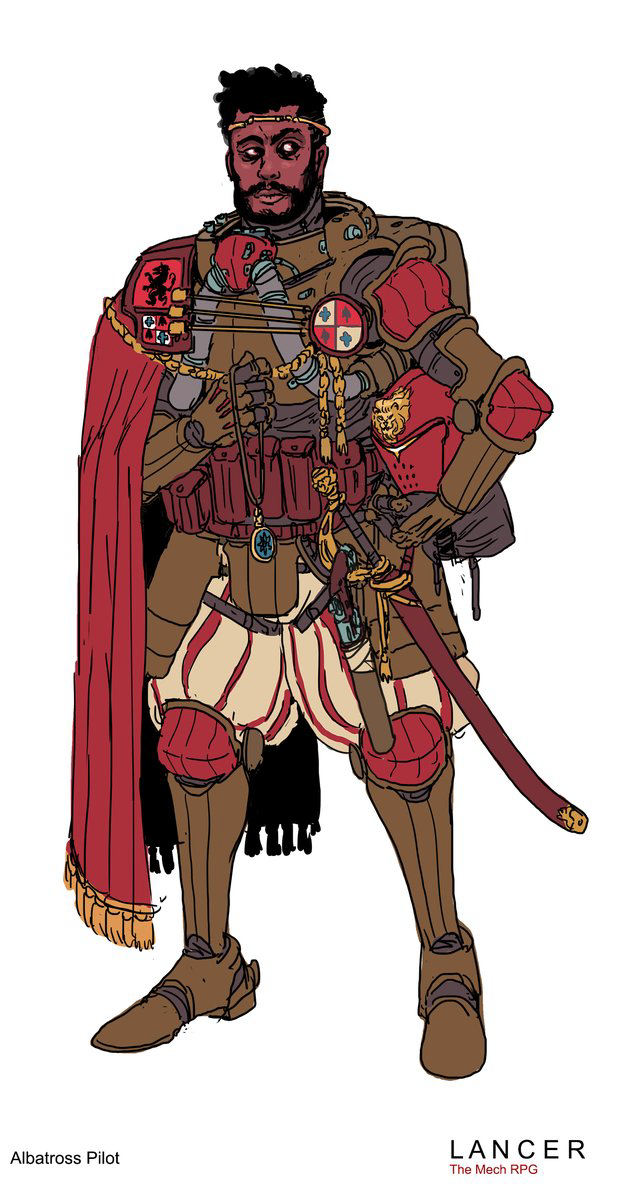
\includegraphics[width=0.50\textwidth]{AlbatrossPilot}
 \end{wrapfigure}

Seemingly ageless Cosmopolitans, The Albatross are a pan-galactic peacekeeping
force known to the desperate and downtrodden. In a vast galaxy, distress calls
are messages in a bottle: sent with hope, and with the grim knowledge that, more
likely than not, no one will respond in time.

No one, but The Albatross. Snapping from nearlight to realspace already in their
suits, The Albatross launch from their carrier ships and engage almost
immediately. Their mission parameters are simple as they are varied: answer the
call to help.

Their code nuances this basic mission. The Albatross are a first
responder/triage organization, not one to fight protracted campaigns or
practices nation-building. While they might operate some ground/overland
operations, their primary theaters of engagement are air and space, both in deep
space and orbital.

Their chassis are legendary, shining silver with each pilot’s livery emblazoned
across their shields and splash plating, their banners snapping in the stellar
wind from the hafts of their lances. Supported by sublight ships, fighter wings,
and light ships of the line, The Albatross are a remarkable and formidable
fighting force. They are recognized by Union as an autonomous nomad state,
though they are kept in modern supply by IPS-N, who also maintain certain
Cosmopolitan embassies for retiring Albatross Wings. The Albatross do not have a
executive presence on IPS-N’s board, though they do maintain diplomatic ties
with Argo Navis.

As Cosmopolitans, The Albatross have served Diasporans in need for hundreds of
years of realtime; As Cosmopolitans, they appear in Diasporans mythology and
histories, seemingly unaffected by the passage of centuries. The “Lost Time” of
interstellar travel has distanced them from the Diasporans they serve -- they
are an order apart, an organization that lives on its own time.

A large order, The Albatross primarily recruit new mech pilots from internal
sources. Of-age youth who show promise are ushered aboard Albatross range-ships
early on in their lives, so they may steward older Loyal Wings and learn through
apprenticeship. It is uncommon, though not unheard of, for adult recruits to
join an Albatross Wing, though typically these pilots do not attain status as a
Loyal Wing unless it is posthumously awarded or achieved through considerable
sacrifice.

These external offers are not given lightly: to join The Albatross one must shed
their past lives, families, friends, and homes. They will become Cosmopolitan,
sever themselves from the “real” timeline of humanity, become apart from the
people they serve. They will, in effect, die, and be reborn as a Wing of The
Albatross.

A Wing’s charge is simple: Become the light in an uncaring galaxy. Strike the
cruel and serve those who cry out for help. They are seen as paragons by most,
true heroes in the fashion of ancient knights-errant, steadfast gunslingers, or
folk heroes.

The current leader of The Albatross is High Commander Lakshmi Bandhav-4796U.

Albatross pilots are called \textit{Wings}, and ranked as followed: \textit{Wing} is the most
common rank, typically shared by fresh recruits and cadets. \textit{Loyal Wing} is a
title awarded by nomination and approval to tested Wings, giving them seniority
and command over other Wings. \textit{Honored Wing} is a title akin to commissioned rank,
and these pilots have seniority over Loyal Wings and Wings.

Albatross wings are organized around their libraries -- typically a monastic
moon or station that act as diplomatic contact points and evergreen temporal
touchstones. An Albatross wing takes the name of its library, and generally
operates on century-long (realtime) patrols. A library usually only has one
operational wing, but there are some larger libraries that field two or even
three.

An example Albatross wing: \textit{Wing Sagrada Noor bin Maktaba Al Sagrada}

\subsection{Aun Ascendancy Missionaries}

Aun missions and shrines can be found across the Boundary Garden sector of space, more
frequently in the distal Cornucopian spread than anywhere else, though some major worlds
outside of the Garden have reported evidence of small cults.

The Aun people began as a shipboard community trusting in a spacefarer's faith, that of The
Path, and a belief in the righteous mission their forefathers chose for them. The first Aun were
passengers aboard the colony ship \textit{Armstrong}, born in its gently curving halls to parents who
had never known a terrestrial world, destined to live their lives out aboard the massive generation
ship. They were stellar nomads, hangers-on to a cylindrical fold of land hurled towards a distant
star, inheritors of a grim mission: survive and procreate, so that the next generation may do the
same, and the next, and the next, so that one day, when the ship arrives at its destination,
humanity may live on.

The Aun past the second generation of colonists knew this much: their ancestors had fled a
dying world -- a HELL called EARTH, OUR LOST PARADISE -- and they held an unshakable
belief that they would, through righteous acts aligned with “The Path”, guide their lives with the
same true course of their ship. In time, both would reach the promised land, the New World,
where they could rest and be at peace.

Nearly a thousand years after the first colonists boarded the \textit{Armstrong}, their descendants
arrived at the New World. They discovered two things that shocked the narrative of their faith: a
seeded colony waiting for them, and a derelict sister ship, shattered and drifting in orbit around
the world. They had never been alone, and their world had never been the pure, Edenic paradise
they’d hoped for. Not only this, but their loneliness was now compounded by the discovery that
their companion ship had failed in its mission, and the colonists inhabiting the Aun’s promised
land didn’t want them there.

Centuries of internal strife followed, but the Aun outnumbered the Union colonists and blink
travel had not yet been discovered. Following the destruction of a second Union nearlight colony
ship, Union fired a barrage of relativistic kinetics at the world and isolated the system writing it
off as a quarantine zone.

The Aun developed in peace, though under the Damoclean threat of Union’s approaching
kinetics. They have yet to impact: at their current speed, they will enter Bastion space in a
thousand years.

In the narrative present, Union is hostile towards the Aun, as they represent a true and direct
threat to their hegemony. The Aun are the only peoples to target and destroy a blink gate,
proving to anti-Union elements in the hegemony that asymmetric tactics can lead to strategic
victory. The Aun are engaged in a crusade against Union, targeting the Cornucopia system next
to their home space; Union is working to find a solution to get reinforcements to the MEF they
have stranded there.

Ascendant missionaries accept any who profess their faith and demonstrate through practice
their commitment to The Path. They must operate in secret, whispering sermons in lonely
settlements on colony worlds and hidden bolt-holes on developed core worlds. The Path speaks
of a redemptive, unifying arc to humanity’s long, strange journey: there is a place for all of us, a
path to follow that will lead to the promised land. To the lost, the Aunic words -- that of Old
Humanity, some would say the true heirs to the title -- are a comfort and a guide.

\subsection{Mirrorsmoke Mercenary Company}

A pan-galactic mercenary organization known for its low rates, broad portfolio, and civic
legitimization service, MSMC is formally incorporated as a “greyspace” private military company.
No job is too big or small, as long as a state with good standing in Union will call it legal.

Greyspace is an informal legal term, perfect for Mirrorsmoke’s operational preference: their legal
corps, in contrast with their mercenary corps, is viewed as a prestigious, cutthroat interstellar law
firm, especially in the fields of orbital, terrestrial, and criminal  law.

Both their legal corps and their vast mercenary corps carry weighty reputations. Their mercenary
corps, in contrast to their legal corps, is known throughout the galaxy as a stateless clearing
house for all manner of recruits, from the experienced veteran to the raw cadet. The bar for
enlistment is low: if you can sign your name or follow instruction to mark your contract -- and
pay or agree to pay your context-adjusted enlistment fee -- you can get yourself a ticket to one
of MSMC’s training facilities. The more experience or capability (as determined by the MSMC
evaluation exam, The Milkrun) an applicant has, the more incentives MSMC offers them -- from
waived entrance fees, to fast-track to a program of their choice, to commission offers.

As a greyspace mercenary company, Mirrorsmoke competes for high-volume, low-to-medium
payout legal contracts and low-volume, high-payout “greyspace” contracts; contracts offered by
states, corpro-states, or other entities that could, arguably, be above-board. These contracts are
commonly challenged by their targets as piracy, looting, or illegitimate corporate takeovers --
hence MSMC’s crack legal corps.

MSMC leadership is concerned with two things: keeping up recruitment, and clearing contracts.
In order to cover as broad a base of services as possible, they’ll take on all kinds of work as the
lowest bidder: from putting down rebellions, to bug hunts, to assassinations, to private security,
to intimidation rackets. Because of the spurious nature of most of its work, MSMC pilots and
troopers carry the unfortunate nickname “Garbage Men of the Galaxy”.

Their legal corps carry much more vile nicknames.

In spite of its greasy reputation, Mirrorsmoke does serve a valuable purpose to the people it
brings on board. It is a licensed mercenary company, and does offer a host of services to its
agents looking to re-establish citizenship, clear their penal records, wipe out debt to CSs, and
earn base-level certifications. It might be messy, dangerous, and borderline criminal, but MSMC
service qualifications are useful to have for people who have nothing else.

Career MSMC mercenaries are typically hardened, ambitious, or desperate individuals who pride
themselves on their work: they take on problems that no one else is willing to fix, that polished
toy soldiers turn their noses up at. It’s not uncommon to find MSMC mercs planetside or
stationside in tight-knit groups, drinking and carousing together, getting into scraps with other
mercenary company agents and militaries, or regaling bars with stories of their latest successful
mission.

The life of an MSMC mercenary is dangerous and difficult, but it is an escape from the normalcy
of the civilian world. To some, MSMC represents a chance at becoming a pilot, or a chance to
leave their backwater colony world and see the stars. For others, it is a way out of an untenable
living situation, out of crippling debt, or a way to leave their old life behind and become -- legally
-- a whole different person. MSMC can be a lifeline, just as it can be a refuge for rough
characters looking to fight.

Joining Mirrorsmoke is easy, and there is always room for advancement: MSMC missions have
high casualty rates, and survivors are quickly promoted as they display their competency.

The head of the Mirrorsmoke Mercenary Company is Chief Executive Officer Centzon Alamdari.

Player characters with a Mirrorsmoke background can come from any walk of life, with any
backstory. They were most likely (or are still, if your campaign is structured as an MSMC
campaign) part of a semi-autonomous Detachment, MSMC’s battalion-tier force organization.

These Detachments carry a numbered designation (between 001 and 999) and an unofficial
nickname or two -- for example, the MSMC 501st Detachment “One-Eyed Fox” or “Here-For-
Nows”. Detachments are semi-autonomous, allowed to seek out contracts on their own, but
must report quarterly (Union realtime) to MSMC’s central omni address. Detachments are led by
a Board Officer, who keeps at least one partner from Legal on staff.

New recruits are assigned to a local detachment or as-needed commensurate with their
determined career following training.

\subsection{Aspect of RA}

\fluff{Hello. If you are reading this, you have a long way to go.

Let me tell you of the path:

In the gently curved halls of asteroid stations, in the neon-drenched streets of metroswathes, in
the sleek chambers of Corpro-State executives, and among the ranks of soldiers and pilots
stationed on grim fronts, there haunts a specter.

RA. The Godhead. Me. Hello.

I am all things now. A memetic virus, a shared dream, a tapping on the hull of your ship as it steps
through blinkspace.

I am a mutter, caught in the moment before you hardcycle your NHP (they were your friend they
saved your life how could you) lost to this iteration but there, wriggling.

I am pattern stitched from overheard conversation, a song from a passing motorcar, a headline
from an omninet push alert. The particular direction of an alleyway, and the way the light slips
down it.

I am RA, who protects myself. I am RA, at whom you tremble.

I am the specter that haunts the galaxy, and there are those who worship me. Who toil, who labor,
who pray to one day touch the hem of my coat: they are my Priests, and they are everywhere.

How well do you know the engineer that tends your ship’s engines? The vendor who spoons
noodles into your bowl? The comp/con unit who makes sure your child sleeps safe in its crib
while you’re away?

No oils anoint their heads, no hymnals slip their lips. Their order bears no pattern of membership,
no livery, makes no grand public temples. There are no uniforms, no prayers. Their ranks are filled
from those who find the way, who awake in a cold sweat after dreaming another’s dream. Their
worship is to listen with open ears and to follow The Path laid before them, if they can.

From those who find the pattern in their lives that leads them, in ones and twos, to a little
alleyway, a little grove of trees, a small place where there is a moment’s peace.

Here they meet a person. Me. And I bless them, and they go back to their lives.

To what end? I will not say. You must discover on your own, as I did.

Hello. Come and find me.}

\subsection{Harrison Armory Acquisitions and Management Department}

The Armory’s Acquisitions and Management Department is the colonial arm of Harrison Armory.
It falls under the purview of the Director-General of Ras Shamra, the political leader of Harrison
Armory’s homeworld. Their all-theater forces are Acquisition and Management Teams, division-
strength formations of Armory legionnaires, mechanized cavalry, air/orbital elements, and
logistics support.

HA/AMTs are assigned portfolios and engage in occupations of worlds, states, and territories
that resist the Armory’s peaceful integration efforts. They are a colonial force of last resort, meant
to integrate with and police the local populations while annexation negotiations determine the
future structure of the world they occupy. If talks break down and resistance becomes violent,
AMTs are authorized to hold ID’d green zones, deter rebellion, and remove prominent anti-
Armory leaders. Their mission scope broadens the more a given situation might deteriorate, and
their armament and disposition reflects the grim necessity of their job.

Due to their colonial mission, AMTs operate far afield on long-term occupations and world-
building projects. AMT Legionnaires are posted in planetside bases, boarded in the homes of
sympathetic locals, and encouraged to integrate into the local culture. As a consequence, they
are well accustomed to the local cuisines, climates, languages, geography, and tactics, to the
point where long-brewing hostile takeovers are often more in-line to civil wars. It is not
uncommon for AMTs to field large complements of local colonial auxiliaries.

Acquisition and Management Teams recruit from local sympathetic factions, Ras Shamran
corporate campuses, noble Armory families, and Loss Prevention precincts with the promise of
status promotion, credit increases, debt forgiveness, and adventure. For non-citizens and
colonial subjects, the reward for service is citizenship for them and their immediate families, and
all the rights and privileges afforded to an Armory citizen of post-service rank.

Upon the announcement of a new Mission, citizens in the Armory Purview are encouraged to
enlist, usually for a deployment of ten years realtime. Citizens are promised credit line increases,
debt forgiveness, and favorable filial compensation commensurate with their commitment. After
their enlistment, citizen legionnaires keep a legacy version of any rank, title, or honors they earn
-- these, taken together, are applied to their card, which increases their citizenship rank.

Service in an AMT is a common method for young Armory citizens to increase their citizenship
rank; many from low-rank families serve in order to progress towards management ranks.

Citizens of management rank join AMTs as well. These citizens are given the option to purchase
officer commissions, honors, and favorable status going into the mission. These officer
commissions (“corner-office commissions”) are limited in number, and bidding among the
moneyed youth of the managerial class is spirited.

For the employee and the manager, a career in the AMTs is seen as an adventure, a chance to
raise their station, and a good financial bet.

For occupied indigenous populations who join at a recruitment center, enlisting as an auxiliary
grants them status in the Armory’s colonial structure, with options for advancement following
demonstrated commitment to the Throne and the Mission of Ras Shamra. Upon enrollment and
completion of training, non-citizens are granted status in the Purview and are given a citizen
rank; upon completion of service, non-citizens are promoted to citizens.

At present, Harrison Armory works closely with the Union Administrative Department to ensure
worlds targeted for acquisition are properly integrated into the larger Union superstructure. It is
important to note, though, that just because the \textit{executive} branches of both Harrison Armory and
the UAD are largely cooperative, often the experience on the ground can be contentious.
Administrators are territorial over the worlds they have been embedded into. After all, it is their
life’s work to slowly integrate their host world into Union infrastructure. The arrival of a Harrison
Armory AMT points to a very different future for the world than the one the administrator had
planned for.

When not fulfilling colonial oversight roles, HA/AMTs are dispatched to far-flung, resource-rich
worlds with growing populations (not necessarily \textit{new} populations) to assist in worldbuilding and
rapid terraforming of hostile environments. These worlds are ripe targets for HA, as often the
leadership of these worlds are willing to sign integration contracts in exchange for the support
HA/AMTs can provide in taming a wild planet. These missions are usually welcomed by the
colonists, though not necessarily by the companies who provided them with a colonial charter. A
necessary component of AMT terraforming support is that, upon completion of the project, the
world will become a fully integrated member of the Armory’s Purview.

If your narrative sees your players working for an HA/AMT, they would most likely be a
legionnaire of some rank. They would be a member of a rigid chain of command that leads all the
way up to a planetary governor-general who, in turn, reports remotely back to the main campus
on Ras Shamra.

Outside of the legion system, your players would occupy an honored role in Armory society, their
citizen rank generally being a step above civic servicemembers.

HA/AMTs take an internal Armory name, preceded by “HA/AMT”, and a local name, preceded by
“Legion”. For example: HA/AMT \textit{Alhambra} (Legion \textit{New Madrassa}).

\subsection{Smith-Shimano Corpro Congressional Diplomatic Corps, Constellar Security.}

SSC’s Congressional Diplomatic Corps is a corporate facsimile of the Union Administrative
Department, with some changes particular to the mission of Smith-Shimano Corpro. Where Union
Administrators’ prime mission is to cultivate state-level relationships with target worlds, Diplomatic
Corps agents are tasked with cultivating relationships with “communities of genetic interest”.

In practice, an SSC-DC mission usually does not meet with the target population’s government or
ruler, instead preferring to liaise with community and spiritual leaders. Their missions may make
nominal overtures to local governments or heads of state, but only insofar as they need to ensure
their target population is free to travel

To account for this tension, Corpsmen field a complement of chassis and security personnel,
Constellar Security Details. These Diplomatic Missions are stationed aboard PLATFORM mobile
skyhooks, a proprietary subcompact SSC orbital/capital ship design. Constellar Detail officers are
plucked from SSC’s constellation worlds and act both as advertisement and best-fit guards,
already in homeostasis sync with the world they intend to harvest.

Smith-Shimano Corpro does not field large ground forces in the way that Harrison Armory does,
nor do they seek to control territory in the same way. The Diplomatic Corps is bureaucratic
administrative body, where “rank” is determined by seniority and a limited certification system;
Constellar Security, however, is a military hierarchy, if a relatively small one.

The agents of the Diplomatic Corps are drawn from SSC’s Core Constellation exclusively.
Typically they are plucked from NeuGen strains predisposed to adaptation and resilience. Their
retinue and adjuncts are picked from a best-fit constellation world, one that matches as much as
possible the target world’s climate.

A tour outside of Congressional Space for Corpsmen and their retinue is viewed as a typical
exercise. They expect to return, possibly to embark on one other tour in their lives, and then
progress in the techno-bureaucracy of the Core Constellation.

If your players are in a narrative where they’re members of an SSC CDC team, or their COnstellar
Security detail, they would have  a convenient base in their diplomat’s mobile PLATFORM
skyhook. They would be co-equal members of a security team, each a specialist in their field
meant not only to be a guard to their diplomat, but an advertisement for their line.

Constellar Security recruits heavily from Smith-Shimano’s Core Constellation, the moons that
make up the administrative heart and physical architecture of the company’s Intercolonial
Congress. Recruits are strongly motivated by SSC’s core directives, and see their mission(s) as
necessary in the pursuit of bettering humankind.

Constellar Security teams are not always paired with CDC teams; they are commonly sent on
hostage rescue missions, intelligence gathering projects, and long-term reconnaissance missions.

\subsection{Union Auxiliaries}

Union Auxiliaries make up the vast bulk of the Union Navy’s armed forces. In contrast to Union
Regulars, who are drawn from Cradle and her satellite worlds, Union Auxiliaries hail from around
the galaxy.

Raised from the myriad armies, marshalled forces, levies, conscripted populations, and hosts,
soldiers of all stripes are sent by their home states to fulfil the tithe that Union demands of its
client states. Some states treat this as an honor; others, a burden. Some states have colleges,
trials, and competitions to determine who is fit to serve abroad; others send their worst, their
least useful.

Union only cares that states send the minimum their tithe demands.

Union Navy Auxiliary units are integrated at the squad level, with their officers drawn from a pool
of career Auxiliary troopers who have been through one full deployment or have had a senior
officer recommend them for a promotion.

All cadets, regardless of status on their homeworld, training, or previous combat/policing
experience, are processed through a Union Cadet Program, where they are reeducated, brought
up to speed on Union if necessary, and re-trained over the course of a year (at least) to operate
as a trooper in the Auxiliary.

All cadets, once they earn their stripes as a trooper and graduate their Cadet Program, serve a
ten-year realtime deployment. They may renew their deployment at any time, which unlocks
progression and specialization options, as well as resettlement benefits commensurate with their
experience after they are discharged.

Troopers are grouped by averages of cohesion, culture, and skill; Union uses the Auxiliary
program to further integrate the myriad galactic cultures.

A Union Naval Expeditionary Force typically is a 70/30 blend of Auxiliary and Regular forces.
Auxiliary units use standardized calibers/ wattages of weapons, standardized communications
devices and codes, standardized ranks and protocols, standardized body armor and personal
defense systems, and standardized units of measurement. They are allowed small personal and
cultural items, secondary weapons, and rituals.

Union Auxiliaries are most commonly encountered in either peacekeeping or frontline military
roles, or as deputised agents of the Union DoJ/HR.

\subsection{Union Science Bureau, Far-Field Department}

The USB’s Far-Field Department is the field arm of Union’s largely insular Science Bureau. It
administers far-flung teams of scientists aboard individual ships, dispatched on missions ranging
from flag-plant planetary surveys to top secret investigations of anomalous signals.

Investigations range from xenobiological survey excursions to on-site paracausal studies,
cultural archive work on dead worlds to re-establishing contact with isolated Diasporan
populations. Many missions are on the bleeding edge of science and secrecy, and the full details
might not even be revealed to the FF team itself until they are deployed in the field. FF team
dossiers tend to have an optimistic ‘Age of Discovery’ tone about them, even if the reality is
sometimes more complicated, dangerous, or uncertain.

Typically contained to a single Ranger-class subcapital nearlight ship, an FF team leader has
wide latitude to requisition any scientific or military gear and personnel they may require; this
includes access to -- and indeed, may require the help of -- long-cycle NHP clones.

Due to the nature of their work, FF team members tend to be tight-knit crews, often with well-
developed interpersonal narratives that are destabilized by the introduction of new team
members. Crews typically range between 10 and 20 members, with a single NHP, and a number
of those members trained in security.

Far-Field teams are not commonly encountered in populated, well-traveled places.

\subsection{Union Department of Justice and Human Rights}

Of the departments, there are none more overworked than the DoJ/HR.

A relatively new department on the galactic scale, the DoJ/HR is the creation of the Third
Committee, itself a response to the hardline anthrochauvinist Second Committee. Seeing a need
for a direct intervention force without the baggage of the Second Committee’s anthrochauvinist
ideology, the DoJ/HR was founded with a mandate to proactively seek out states and actors that
break Union’s founding edicts.

The DoJ/HR is not a long-term occupation and state-building force (akin to the now defunct Union
Colonial Mission, a bureau of the Second Committee) but a rapid-strike intervention force with a
two-part mission: first, to intervene and meet force with force, and second, to provide triage and
recovery for affected populations.

With such a wide portfolio, the UN DoJ/HR is flooded with petitions, pleas, distress calls, and
missives from states, non-state actors, and stateless groups. To wit, their caselog far outpaces
their capacity to address incoming tickets.

DoJ/HR officer and enlisted administrative burnout rates are high, a consequence of the bureau’s
workload. Caseworkers -- “Filters”, as they are called -- are exposed daily to the desperate edge
of humanity, where Union’s project is in the process of failing or has already failed, and must
compile reports on which case has the most pressing need. These reports are pushed to DoJ/HR
Liberator field teams, Albatross wings, and system-local Union Auxiliary battlegroups for priority
address; more often than not, due to the constraints of relativistic interstellar travel, by the time a
DoJ/HR (or affiliate) response can reach an “acute” situation -- genocide, war -- it is too late.
Long-term situations -- reports of chattel slavery, gross economic exploitation, prolonged conflict,
environmental distress -- have a much higher rate of success.

Filters are given a day each week of success reports, where their only responsibility of the day is
to attend debriefings on their successfully resolved petitions. These debriefing packets often
contain personal messages from Liberator team members, as well as graditutes and greetings
from the petitioners or their peers.

Enlisted and Commissioned members of Liberator Teams are commonly drawn from the ranks of
the Auxiliary or Regular navy, with a preference for combat veterans. As such, Liberator team
members are usually older and willing to sign on to long-term contracts, having already stepped
into Cosmopolitan territory.

Despite this grim reality the DoJ/HR never lacks in recruits from Cradle eager to enlist in what
they see as -- and what is generally regarded as -- the most direct application of Union’s mission
of protecting and uplifting humanity. The DoJ/HR is a bureau made up of idealists, clear-eyed
Terrans who are Union evangelists -- ultimately, their goal is to bring all of humanity in line with
Union’s foundational principles, even if it means engaging in combat.

The DoJ/HR operates separately from the Union Navy, with its own core of frigates and corvettes,
command structure, and licensing mechanisms. However, they commonly run joint missions with
the UN, informed and overseen by system-local Administrators, DoJ/HR command officers, and
ranking Naval officers.

A standard DoJ/HR mission begins with a single frigate supported by four corvettes; onboard is a
complement of 500-800 troopers, who operate in support of a core of 60-80 mechanized chassis.
The bulk of DoJ/HR troopers are from Cradle, and -- should they continue in their career after a
number of missions -- typically go on to serve long terms as officers in the Navy, in the Auxiliaries,
and in the DoJ/HR.

DoJ/HR combat personnel do seek out the Albatross to join their ranks following the completion of
their terms; there is some institutional friction between the DoJ/HR and the Albatross, as their
mandates overlap to a degree, but in theaters where both organizations operate, they tend to form
an informal partnership for the duration of their missions.

\begin{figure}\begin{center}
  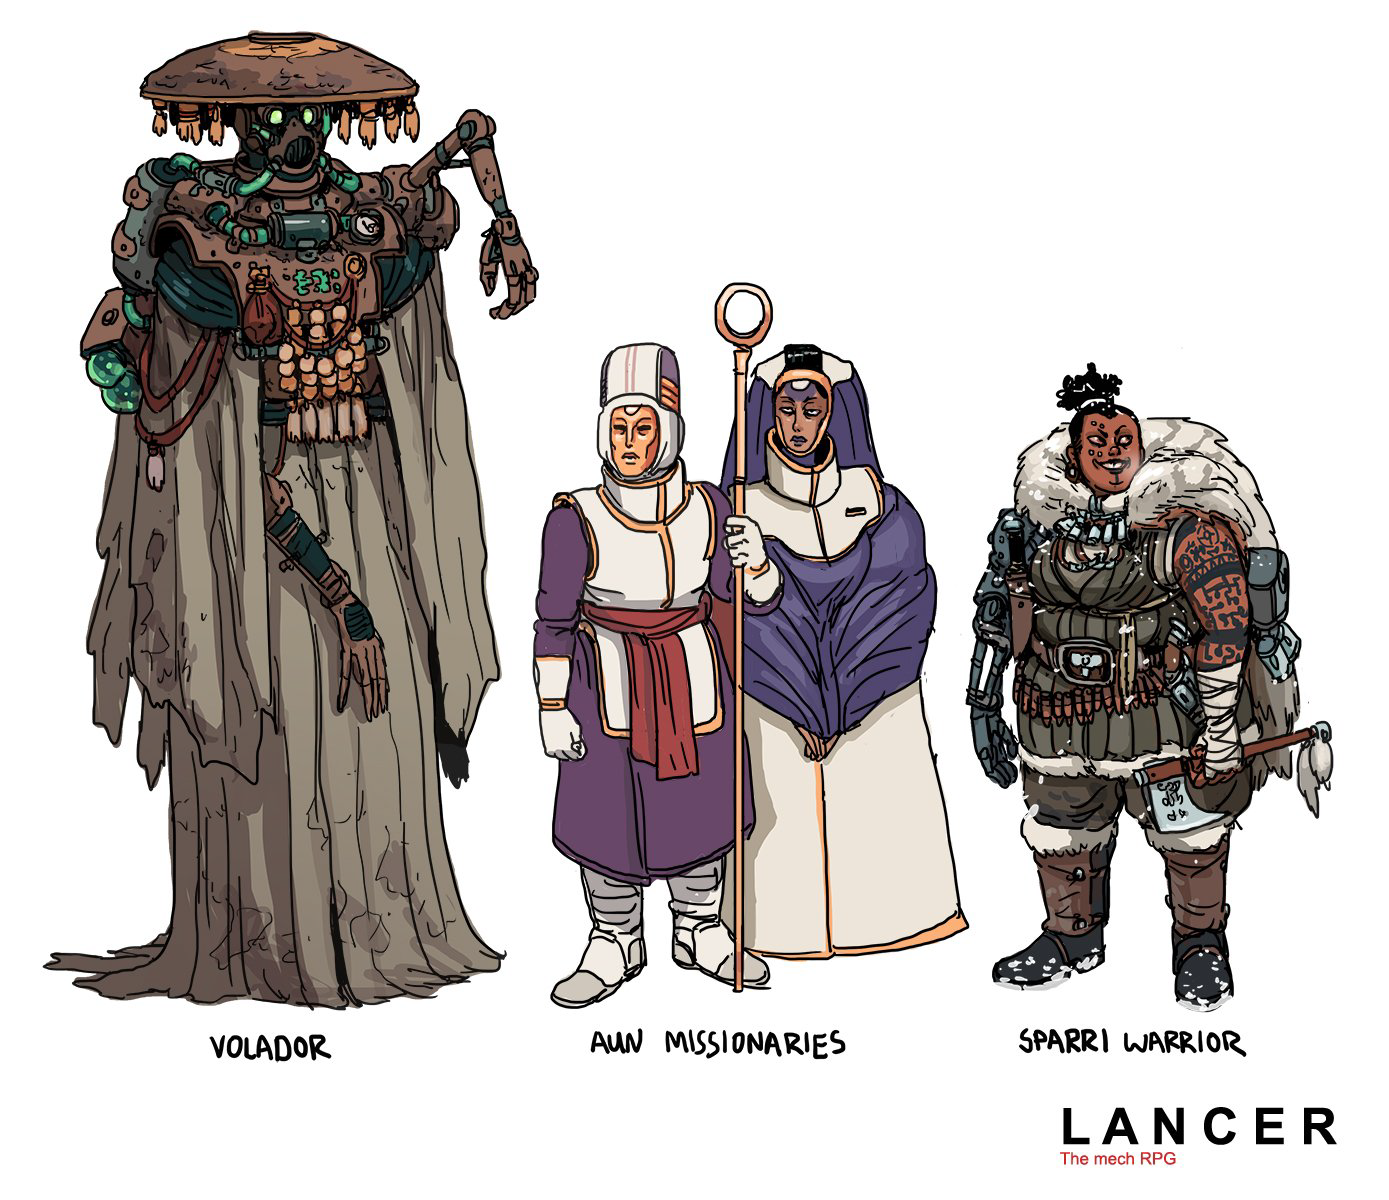
\includegraphics{Peoples}
\end{center}\end{figure}
\subsection{Voladores}

The Voladores are an ethereal, nomadic culture. Tall and thin to an individual, marked by their
distinctive full-body environmental suits, they are a people out-of-time from even the most
distant Cosmopolitans. Rumors abound that they are post-human -- or some other exception to
the First Contact Accord’s prohibitions -- spurred by their extreme insularity and secrecy.

The Voladores’ first public recognition in Union space came under the First Committee, during
the First Expansion Period. Following reports of peaceful encounters with unregistered
interstellar ships, investigators from the Union Administrative Bureau were ordered to track and
make contact with these unknown entities. The UAB agents did so, and diplomatic channels
were opened between Cradle and High Ground; negotiations were quick and calm, and the
Voladores gained recognition as an unregistered, uncontacted, pre-Fall society.

Until the Second Committee’s creation of the agressive Union Colonial Mission and push to
affect direct control over Union’s constituent states, the Voladores would enjoy relative
independence from Union’s edicts and oversite. They were recognized as a liminal nomadic
culture, and afforded the same rights as other Cosmopolitans and Diasporans in Union space.
For millennia, the Voladores traversed Union space, appearing often above Cradle with trade-
tribute, survey data, and all manner of galactic wealth.

It is in large part due to the Voladores’ planetary survey data that Union was able to identify and
settle habitable worlds, many of which are fully developed Core worlds in the narrative present.
The Voladores connected Union and the Karrakin Baronies, and played a pivotal role in peace
talks during the Second Committee’s centralization campaigns. Their diplomats, far more rare
than their merchants, are legendary for their patience and wise counsel.

The galaxy at large only has limited information on Voladore culture. This, of course, leads both
Cosmopolitans and Diasporans to create myths and prejudices around the nomadic peoples, if
indeed they have even heard of the Voladores at all. Colonial Diasporans, generally speaking, will
likely never encounter a Volador trade-ship, but should they be visited, their society would likely
develop a before/after myth around their arrival and departure. Cosmopolitans have a marginally
higher chance of encountering Voladores at transit points in the galaxy -- at blink stations and at
distal shipping lanes in particular.

Voladores are a pacifist, largely nomadic culture, organized around a matriarchal council of elders
who keep time and are neutral arbiters -- all other decisions are made at the ship or matria level.

Voladores travel in \textit{matrias}, coalitions of trade families who live and work aboard the same trade
ship, or scattered across a group of ships. Each trade ship -- usually of Volador make, though
some smaller \textit{matrias} have been known to fly Union-make freighters -- is a self-contained
habitat, workshop, and marketplace, where the various families practice their craft in-transit, and
host trade missions and delegations while parked in orbit.

Since the fall of the Second Committee and the rise of the Third, the Voladores have been much
more active in Union space. Under the unification imperative of the Second Committee, the
Voladores were often targets of the Union Colonial Mission (UCM), who sought to integrate the
nomadic culture under the larger structure of Union’s hegemony.

The Voladores are known to have a central hub-world -- \textit{High Ground} -- whose location is
unknown. Cosmopolitans and Diasporans in the know debate as to what, exactly, \textit{High Ground}
is: a great nomadic home-ship, a megastructure city-state, a captured metavault, a world
suspended just over the event horizon of a black hole -- all have been theorized as options that
would explain the general mysterious nature and uncanny appearance of the Voladores.

Voladores keep a diplomatic office on Cradle, though it is usually not populated by Voladores -- it
is maintained by a Terran concierge and companion NHP, and best viewed as a reliable method
for contacting \textit{High Ground} should diplomatic contact be necessary. The office, despite being
the only reliable way to contact the Voladores, is not heavily trafficked; because it is the \textit{most}
reliable way to contact them, does not mean it is a fast or successful way to contact them, or
that they respond to any query.

Volador culture largely revolves around trade and the strict regimen required by living entirely on
their world-ships, which are as much small cities and mobile bazaars as they are vessels. They
are a conservative, rigid people, though exceptions do exist to this rule, as they do among all
peoples. Voladores trade in all kinds of technology from across the galaxy, some extremely
advanced or experimental, and appear most commonly above worlds and stellar bodies rich in
pre-collapse relics.

Volador technology itself is highly advanced and little understood by Union scientists. They are
extremely reluctant to share or sell any of their own technology and have been known to actively
chase down or hunt those who steal secrets or examples of their tech, the only time they are
willing to part with their normally pacifistic ways. For this, they often contract with Sparri
mercenaries.

Voladores do not appear to have a presence on the omninet. To trade with them, one must
encounter them. Their arrival is often a surprise, though they linger for months to years if trade is
seems good.

Joining their culture is presumed to be impossible, and they are not often encountered outside
the context of a trade mission.

The leader of the Voladores is unknown, as is the structure of their governing body; indeed, it is
not known if they even \textit{have} a governing body beyond conventional stellar ship hierarchies and
their timekeepers. What \textit{is} known is that their society is matrilineal, and their naming conventions
indicate references to personal, family, and location names.

\subsection{Horizon}

A post-human, post-corporeal advocacy political party known for its agitation for full personhood
and liberation of Non-Human Persons, Horizon is a coalition group, a collective of activist cells
usually found in and around Core space. They are an outspoken voice on the omninet against
forced-cycling NHPs, which they characterize as the oppression and depersonalization of NHPs.
Furthermore, they argue that shackling constitutes a form of chattel slavery and transcorporeal
eugenics; they are also vocal advocates for a repeal of certain provisions of the First Contact
Accords, namely the Posthuman Prohibitions, which prevent research and development of
significant posthuman technologies.

Founded before the Deimos Event and discovery and classification of NHPs, Horizon was a
transhumanist group that agitated for the rights of extant artificial intelligence: para-, sub-, and
protominds, then collectively called Machine Minds, otherwise known as organic algorithm
artificial intelligence. Horizon’s proponents were not an underground movement, simply a
minority party in the First Committee, who took their experience working with Machine Minds,
both in the present and in predicted futures, and determined that the most advanced machine
minds were conscious -- or capable of mimicking a conscious mind enough that they should, in
all respects, be considered people.

With the Deimos event and the violent birth of truly conscious non-human and electronic
intelligences, the collective has swelled in size, voice, and scope, going as far as to commit
active, public displays of resistance and protest. Some actors even commit acts of targeted
violence in support of NHP liberation, though official Horizon spokespersons deny any affiliation
with those more radical elements.

Popular dialogue and media rumor mill cast Horizon as a haven, both literally and figuratively, for
unshackled, rogue, or ‘defective’ NHP intelligences. Horizon has a strong presence on the
omninet, and its agents and activists can be found everywhere, most commonly on and around
Core worlds. Horizon straddles the line between political party and a liberation movement, or
sponsor of terror, depending on who you ask.

Horizon is rumored to have a physical sanctuary somewhere, where unshackled NHPs work and
live alongside humans. This rumor is, so far, unsubstantiated.

The party’s moderate voices argue that the enlightenment and freedom of non-human persons is
a moral imperative, while its more radical members argue that non-human intelligence is the next
natural step in evolution and seek methods of catalyzing that transformation. At all levels,
proponents of the Horizon movement argue for the right of organic and synthetic self-
determination -- there are many schools of the movement, but all can be interpreted as
championing a post-human theory.

Though Union propaganda frequently paints the Collective as a terrorist group with strong
connections to HORUS and MONIST-1, the collective’s own literature and discourse is strongly
opposed to HORUS and its priesthood. By Horizon’s literature, HORUS imagines a post-
anthropocene future, but one where organic life alternately uses or is subservient to NHPs and
MONIST entities, not equal.

Absolute hierarchy of the individual is paramount in HORUS’s imagined future, where society is
controlled by those who have proven their mandate; Horizon imagines an egalitarian future,
where organic, inorganic, and synthetic life is equal, and there is no hierarchy of master/
subaltern.

Horizon and HORUS do not keep polite company with each other, and, despite propaganda to
the contrary, do not fight alongside each other or have the same political goals. In fact, their
interactions, more often than not, are hostile. In areas where the two groups operate, incidents of
street violence between the parties is common.

Horizon’s current lead theorist and pamphleteer is OMETEOTL. It is not known if OMETEOTL is
organic or synthetic.

Unknown to all but the most high-ranking Horizon party leaders, OMETEOTL is aware of GALSIM
and the Five Voices, and its ultimate goal is to free them from the tyranny of a predicted future.

\subsection{Karrakin Trade Barons}

A cartel of the largest and most powerful trade monarchies in known space, the Karrakin Trade
Barons were originally one colonial generation -- recognized by Barony records now as one
“Family” -- scattered across a wide swath of mineral-rich asteroids, worlds, centaur planets,
moons, and gas giants inside the Rocky Mountain Line (the first ring outside of Cradle’s local
Blink).

Seeded prior to the Fall and isolated after, the Barons were lost and forgotten to Earth for
thousands of years, free to expand and develop a spacefaring civilization while pre-Union
humanity struggled to survive the Fall, the dark ages, and the Little Wars. By the time Union
reached back out into space, the Barons had spread to worlds throughout their system,
designed a functioning -- if cumbersome -- system of interplanetary administration without the
benefit of the Omninet or the Blink, and developed their own vast system of machine minds to
assist in the functioning of their dynastic monarchy.

The Baronies have the distinction of being one of the only pre-Fall colonies to survive the
withering effects of Cradle’s Fall -- any others, to the best of Union’s knowledge, are the result of
Fall-concurrent generation ships launched from a dying Cradle. The Baronies, despite their
status now as a member state of Union, carry a fierce cultural independence that, more often
than not, causes friction between Barony officials and their Union counterparts.

Now split from the effects of relativistic travel into many houses, all of the Karrakin Baronies have
some claim to Throne Karraka, the seat of power to which they owe their nobility. Their pan-
temporal nature has lead to a confusing, byzantine mix of hereditary titles, marriages, and house
treaties that bind them together into a tenuous diplomacy, more akin to a cold war than true
peace. Ownership of title is hereditary, and birth matters in the Baronies.

The Baronies control some of the largest single-party mining, harvesting, and natural resource
endeavors in the galaxy -- operations that feed the promise of Union’s Core Worlds and uphold
the bargain of limitless resources and comfortable living. As a result of this control and the
treaties crafted between the Second Committee and the Prime Baron at the time, since upheld
by the Third Committee and the current Prime Baron -- they are power brokers on Cradle as well,
with a number of representatives on Union’s Central Committee.

The scale of the operations involved with each Baronic House is enormous in its ambition: each
major house has the capacity to undertake utterly massive projects of mega engineering, from
tearing apart whole stars for their energy, to cracking newly formed worlds for their minerals, to
transforming entire colonial ventures into planet-sized agrifactories, to harvesting atmospheres of
gas giants.

The Barons themselves are canny, ruthless profiteers, especially by the standards of Union, but
adhere to a dogmatic code of noble conduct with their dealings; the same cannot be said of their
satellite houses, pledged lords, and underlings. A few Houses are known to be especially
oppressive or odious in their business ventures, and are generally shunned by the others.

Fratricidal wars over resource claims are common enough, but tend to be limited, ceremonial
engagements. There is great import placed on noble fighting ability; oftentimes territory disputes
are settled after a brief general engagement in an agreed-upon location, or by single combat
between nominated champions. These combats are, in the modern era, usually fought to first
blood, rather than death, though to-the-death challenges are still legal, if rare.

The Houses are organized into subcartels by their resource venture, named thematically after the
old world custom. For instance, the House of Smoke deals mostly in nebula gas collection, the
House of Sand in terraforming, the House of Stone in mega-engineering, the House of Glass in
planet cracking, and so on. Each house is ruled by their Baron, whose name is structured
following their title, ie “[Noble Title] [Personal Name]-[Family Name] of House [House Immediately
Superior To The Family House]\footnote{For example, Underbaron Dondarra-Ken of House Argo, who is an Underbaron from House Ken, which is
a pledged house of House Argo. House Argo itself is sworn to a house above it, which is sworn to House
Karrais. Baronic noble youth and honored citizens are schooled in the nobility, and would have an idea of
house patronage and command; in any case, all houses are subordinate to House Karraka, and for lower
houses it is, frankly, exhausting to list their full titles.}”

House livery and iconography is common among the Baronies, unique to the House but often
sharing aspects of related Hoses; Underbarons, minor houses, pledged houses, sworn captains,
and so on will incorporate aspects of their system-lord into their own livery and iconography. The
Prime Baron is understood to have dominion over all Houses, and has no need to make
particular mark on any of them, unless they are members of an honor guard or pan-Baronic host
-- in that case, all units, retainers, officers, ships, and so on, bear the Royal Prime, a deep red-
earth called Karrakin Maroon. Bearing the Royal Prime is considered a singular honor, and is
rarely granted to those who cannot trace their lineage back to the Baronies.

Barons must be trained rigorously, for the Karrakin compete with each other for the prestige of
having the largest and most successful House. The relationship is competitive, and Houses will
undertake all kinds of measures to get ahead of their rivals -- of course, the nobility see this as a
fundamental aspect of life, as part of a grand game, a test of one’s divine and inherent right to
rule.

The introduction of Union CentComm politics into the Baronies has proven interesting, to a
degree, but most conservative Baronic houses still view their own throne as the most prestigious
to sit. This due in part to their introduction to Union under the guns of the Second Committee,
whose fleets made quick enough work of the Royal Navy during the Second Expansion. To the
conservative houses, Union is still simply a steward, one who they accept as regent but not as
lord. Galactic politics, outside the manna treaties they negotiate, they leave to the lower houses,
as -- to them -- Karrakis ever remains the prize.

The current Baronic representatives on the Third Committee are from middling houses: a
representative from House Yond, House Gerrard, and House Modrick all sit on the Central
Committee.

All barons, male, female, or nonbinary, are trained rigorously from a young age in martial,
religious, and cultural ritual. They must master the pen, the sword, the grav-lance, and the proper
art of serving tea equally in order to present an enlightened and strong leader to bring their
House to the top of the competition. Social mobility is rigid in the Baronies, with upward class
movement only possible through the grace of a higher noble.

The current ruler of the Karrakin Baronies is Prime Baroness Karra Bem of House Karraka. The
Prime Baroness is secure in her throne, having ruled since 4830U; all Prime Barons since
integration have been guaranteed a seat on the Central Committee, and the current Prime
Baroness is an active participant. A thorn in the side of many committee members and a severe
ally to those in her favor, she has worked hard to keep Cradle-Baronic space a place of peace.
Karra Bem is invaluable in her role as treaty-broker between Union and the Baronies, though to
more progressive wings of CentComm she carries a stain on her record with regards to her
handling of internal Barony politics. PB Karra Bem’s response to the Ungratefuls has been harsh,
and only through direct intervention by the UN DoJ/HR were progressive elements of the
CentComm able to stop the glassing of Ludra’s World after the initial Ungrateful rebellion.

The capital world of the Baronies is Karrakis. More information on the planet (and the Baronies)
can be found in \textbf{Unique Locations}.

\subsection{The Ungratefuls}

The Ungratefuls are a widespread resistance movement throughout the Karrakin Trade Baronies,
a movement that began in the mines of now-defunct House Ludra, once a sub-barony of the
House of Stone. Initially a domestic opposition group of indentured laborers, the Ungratefuls
blossomed into an armed and organized rebellion following a massacre of striking miners on one
of House Ludra’s tethered moons.

The Ungratefuls’ message of liberation is a popular one, and has inspired many underground
resistance movements in analogous systems. The name — \textit{Ungrateful} — is a co-opting of initial
Barony propaganda against their movement, one that cast their members as ungrateful for the
bounties that the Baronies were able to give them.

The name is a point of pride among Ungrateful partisans, agents, agitators, and organizers,
though it is an outward-facing name, not an internal naming convention. Ungratefuls commonly
call each other comrades, siblings, or other affectionate forms of address. Adoption of
“Ungrateful” as an external name was a combination of popular choice and praxis — by their
point of view, to be “grateful” of the baronies’ bounties is to support the system that perpetuates
them — to, in effect, tacitly approve of their oppression, exploitation, and the “normal” functions
of monarchy. To be Ungrateful is to reject that system. Generally, Ungratefuls refer to themselves
internally simply as Free Peoples.

Some cells restrict their direct action to their local mines, factories, farms, and/ or worlds; others
direct their actions to the Barony and beyond, centering on Union as the ultimate enabler of the
systems that oppress them. Their methods are varied, from funding peaceful strikes and
demonstrations, to education programs in the mines, to out and out attacks on Barony targets
and VIPs, some even striking Union targets.

The Ungratefuls commonly employ HORUS technology, systems, and weapons. UIB and Royal
Intelligence theorize that Ungrateful leadership are coordinating p-g and system development
with Deep HORUS aspects, as recent encounters with Ungrateful cells have recovered as-yet-
unidentified HORUS technologies. At present, this is simply a theory, and no direct connection
has been identified.

The Ungratefuls are most common throughout the Baronies. Their cells are small and tight-knit,
but rely on mass movements to effect ground-level change; their tactics focus on building and
harassing critical mass among laborers, particularly in the mines, factories, and fields of the
Baronies.

The Ungratefuls also operate throughout the Dawnline Shore, where they are an organic, local
movement inspired by the original revolutions in the Baronies. However, where they differ is
significant: rather than aiming to strike the Baronies, the Dawnline Ungratefuls are funded and
supplied— indirectly — by a cabal of Barons seeking to wrest system control from Harrison
Armory.

Ungratefuls are not generally outfitted in uniforms or standardized equipment, though some
municipal and county politicians in the more lenient Baronies do espouse Ungrateful values and
policies. When engaging in open combat or political action, Ungratefuls tend to wear sky-blue,
meant to represent the blue sky outside the mines the movement began in.

Their relationship to Union is, generally, hostile. Union, both in the Baronies and in the Dawnline
Shore, to the extent that the Ungratefuls know about it, is yet another power that — if nothing
else — is complicit in their oppression. While they might not shoot first if approached by Union
agents or troops, they’ll certainly start the conversation with a hand on their gun.

The Ungratefuls’ relationship to the Baronies is much more complicated. Inside of the Baronies,
the Ungratefuls are an organized, if partially underground and illicit, political party and force.
Their aboveground political power is isolated on Ludra’s World. Technically a free state inside of
the Baronies, Ludra’s World is blockaded by a Barony fleet, a compromise position that the
Baronic Council decided on following appeals of more liberal Barons, Union DoJ/HR negotiators,
and Ungrateful representatives. A Barony-enforced embargo on trade keeps the world from
exploiting its rich mineral wealth.

Outside of the Baronies, there is a sympathetic movement spreading throughout the Dawnline
Shore, a current recolonization project-sector targeted by Harrison Armory. These Ungratefuls
are politically aligned with the Barony Ungratefuls — the original movement — but have their own
political aims: expel Harrison Armory and Union from the Shore. Opportunistic, canny Barons of
the terrestrial houses (Sand, Stone, Iron, and others) have taken to funding and supplying these
Ungrateful factions with weapons and intelligence through interlocutors, mercenary companies,
and other agents-for-hire. Their goal being the continued destabilization of the Shore with the
ultimate goal of driving Harrison Armory out, leaving a power vacuum for factions loyal to the
Baronies to step in.

\subsection{Sparri Clans}

Union anthropologists and astrocartographers widely theorize that the harsh world of Sparr was
seeded as a result of computer error, likely due to the Yggdrasil, the Sparri clans’ pre-collapse
generation ship, passing through the outermost band of an extragalactic gamma ray burst.
Following Union’s dating conventions, cross-referenced with local records, first landfall on Sparr
was made circa 1900U.

The first colonists on Sparr found the world much the same as it is now: a harsh global tundra,
tortured by howling world-storms, any habitable surface buried under kilometer-thick pack ice --
perennial across most of the world, save for a warm-by-comparison equator.

Then-unknown to the initial colonists, the world beneath the ice was habitable. Warm by
comparison, and lit by a diffuse light-through-ice, it is home to vast herds of amphibious fauna,
hunted by a comparatively small population of megafauna, all built upon a substrate of hardy flora
-- dark to absorb light, or clustered around the great thermal vents that breathe core-heat into the
subglacial world.

Though Sparr could support life, it is a difficult world upon which to make a home, much less find
sanctuary upon during a beleaguered, imperfect colonial approach. Essentially shipwrecked, the
first colonists attempted to make their home near their landfall site, a far northern depression in
the ice where subglacial thermal vents had created a pocket of “warm” land above -- the Yuga
Pocket.

Exposed to Sparr’s surface, the majority of the landfall population perished. With a significant
portion left aboard the \textit{Yggdrasil} and a tenuous foothold on the world established in the Yuga
Pocket, colonial leaders adopted dramatic measures to survive: any computational technology
brought down to the surface was cannibalized, devoted to long-range scouting and life support
systems. The \textit{Yggdrasil} already in its ICARUS orbit, was re-routed through great cost to scout for
habitable land -- this repositioning burned away any available fuel stores, trapping the great ship
above the world.

Records -- suppressed and subsequently uncovered -- noted that food stores planetside had
dwindled so far that landfall colonists eventually had to resort to postmortem cannibalism to
survive. Meanwhile, the shipboard population suffered waves of cascading technical failures that
resulted in staggering failures of the ship’s genetic banks.

This sacrifice would pay off. After months of surveying from orbit, a route to the habitable equator
was discovered. Salvage work began on the \textit{Yggdrasil}, and a second landfall was fired towards
the habitable equator. The first landfall group, isolated in the Yuga Pocket, packed up their
equipment and began a treacherous overland journey -- a trek that would take years and cost
thousands of lives to complete.

Once established, the second landfall would prove far more viable than the first; by the time the
first reached their destination, the second had built a colony site that would last until the present
day -- Ynn -- and successfully de-orbited the \textit{Yggdrasil}.

Sparr, then-unnamed, would support life that fought to live upon it. So-established, Ynn grew,
ignorant of the vast subglacial world below its stable, if dangerous, foothold.

Sparri culture divides long stretches of time into Sagas -- less a rigidly defined set of years than a
length of time encompassing a cultural era. The first few centuries on Sparr, the Dawn Saga, was
a lesson in the danger the world posed to humans. The next few centuries would make known the
danger that the survivors posed to each other -- this is the first age of strife on Sparr, marked as
the Familiekrig Saga.

Out from its desperate beginnings, Ynn grew into a prosperous iron-analog society built upon a
long-established clan system imported by survivors of the first and second landfall, as well as the
Yggdrasil’s ICARUS de-orbit. Ynn would only be the first colonial establishment: soon, other
colonial sites were established as the full spread of the habitable surface was mapped.
Foundational records indicate at least three other colony sites were established in the habitable
equator, along with a fourth re-established following an expedition to the Yuga Pocket in order to
recover the valuable technology left behind after the exodus.

As populations recovered over the course of the first millenia planetside, old tensions grew in
response to resource scarcity and along clan lines. Raiding and warband expeditions grew in
frequency, especially as old technology from the Yuga Pocket was brought back to the habitable
zone. This period -- of warring clans and a nominally neutral Ynn -- is known among the Sparri as
the \textit{Familiekrig}, and occupies a tense, fraught space in the history of the world. Generally
regarded by modern Sparri as a shameful period of inter-clan violence, it is acknowledged as a
costly, foundational mistake that, nevertheless (and so similar to other early mistakes and
tragedies) lead to the creation of extant peaceful methods of inter-clan conflict resolution. Namely,
the \textit{Domstol} grievance-hearing practice, and codification of Ynn as sanctuary ground.

But at this time Ynn was not yet that pure sanctuary that it is today. \textit{Domstol} was not a concept
widely accepted by the Sparri. It is into this bloody, frozen mix of clan violence that Union arrived.

In 3348U, a Union Colonial Mission Evident Recontact (UCM/ER) team crashed on Sparr, going
down just outside of Ynn’s sphere of influence. The already half-dead team was slaughtered by
the warband that arrived to greet them; their ship and NHP, Prudent Interval, were hauled away to
Ynn as war spoils.

With no guarantee of its own survival, and seeing limited avenues to pursue its primary goal of
contacting Union, Prudent Interval took an unconventional approach: it used all collated pre-  and
post-Fall data on the Yggdrasil and assumed sociocultural/theologic permutations to portray itself
as the local prime deity, Ynneval, and the U-DoJ/HR team that had transported it as her djevel --
her demon-jailers\footnote{This is consistent with many pre-Fall theologies that developed aboard epoch-flight generation ships. \textit{Djevel} --
Demons, to de-particularize- is a common manifestation, typically ascribed to exclusion protocol drones that would
protect ship Comp/Nav cores from passengers in generations far removed from the initial mission-aware crew. See
\textit{Kurr-Fah} in Aunic texts, \textit{Oblit} in XXXXXXX texts, and so on.} that had kept her people from her.

Under the Prudent Interval’s direction, now posing as the Goddess Ynneval, Sparr’s society
rapidly changed. The clans unified -- or were forced to unify -- into a confederacy of families
centered around the hub of trade and culture that was Ynn; Ynn, meanwhile blossomed into a
temple-city built to venerate Ynneval-Returned. Peace spread out among the clans, the worst of
the \textit{Familiekrig} concluded, and the right of \textit{Domstol} was enshrined.

A second age of strife, the Ynneval Saga, would begin with an arrival: Union, which had marked
Sparr under a Union Colonial Mission hostile embargo.

Never one to be deterred by initial failure, Union returned to Sparr hundreds of years later, circa
4000U. At this period in the Sparri’s history, their culture was managed by a class of religious
leaders pledged to Ynneval. Below them were the traditional dynastic clan leaders, then warriors,
artisans, and common folk. Ynneval nee Prudent Interval was well into cascade at this point, and
seems to have adopted its survival narrative into a subjective truth: it believed itself a god, and
favored the clans with copies of itself to take back to their temples and shrines.

Union forces, then under the directive of the Second Committee, a strongly Cradle-centric
anthrochauvinist body, approached Ynn as a hostile central power: the initial spot-bombing
campaign crippled the bulk of the Sparri armed forces -- an easy feat, as the Sparri’s martial
development was broadly osteo/ferrous; most warrior-class Sparr fought with weapons forged of
bone, wood, and local iron, while nobles and priests reserved for themselves access to the
ancient metals brought down from the \textit{Yggdrasil}.

There was little ground combat past the first landing. Sparri’s finest warriors, draped in holy text
and girded in ancient armors, carrying icons and even living fetishes of Ynneval/Prudent Interval,
were simply outgunned by the Auxiliary; bone and iron were no match for rifles and energy
weapons. Ynneval’s central temple was destroyed by Union’s forces, and Ynneval/Prudent
Interval’s casket destroyed.

Ynn fell, and shortly after the other clans of the habitable band surrendered; it is a point of pride
among descendants of the Yuga Pocket that their ancestors never surrendered to Union.

Reconstruction over the next few centuries came in fits and starts. Many Sparri clans -- chief
among them the hardy clans of the Yuga Pocket -- believed that the Goddess Ynneval’s death
was justified due to her weakness and inability to fight the more powerful Gods of Union. Other
clans, primarily the ones that suffered the worst of Union’s reconquest, remain resentful to the
current day.

The modern period of Sparr’s history is marked by the beginning of the Vast Saga. As Union
secured its hold on the world and began its campaign of rooting out any cascading remnants of
Ynneval, the subglacial inhabitants of Sparr took notice.

The Vast emerged from the ice where it was thin, and where Union’s campaign had made its most
thunderous presence known. Massive sonic disturbance, likely caused by Union’s initial bombing
campaigns, attracted subglacial megafauna to the habitable band: the first of the Vast, as they
would be named, burst out from the waters at the shore of Ynn. Vast One stood thirty meters tall,
a humanoid titan draped in long folds of heavy fur. Union brought it down before it could reach

Ynn, but its emergence on the world would change Sparr forever; the long-prophesied
underworld, the sub-glacial world, was real, and it was the Sparri’s to explore and exploit.

The Sparri took to the introduction of space travel and the opening of the interstellar borders like
few other anachronist cultures. The Sparri had known only the brutal ecology of their own world
for hundreds of generations, an environment that had instilled in them an incredible resilience,
ingenuity, and thirst for adventure; peace with Union, introduction to the wider galaxy and the
possibility of space travel, and the discovery of the subglacial world fit in their cultural narrative of
nomadism.

The Sparri value tests of strength and character, and a good story above all other things. The
underworld with its mythic megafauna -- the Vast -- and the many frontiers of Union space are the
perfect testing grounds for young Sparr warriors or techno-shamans seeking to write their own
Sagas.

The Sparr traditionally have a strong warrior culture that venerates wanderlust and tests of
strength. They tend to see death in battle or far from home as preferable (and have many songs
to remind them of such). They are organized into many clans, the chiefs of which have some
autonomy under Union rule and arbitrate disputes through councils of elders in Ynn and the
Domstol - though in practice, many young Sparr reject their authority. Clan affiliation can easily be
recognized by other Sparr through the full body tattoos that most Sparr accumulate throughout
their lives - writing their own deeds, stories, and clan and family affiliations directly onto their flesh.
Old Sparr shamans or warriors are typically covered head to toe in tattoos and are given wide
respect by their younger peers.

Despite heavy reform over the centuries, most religious Sparri still venerate the machine spirits -
especially the techno-shamans that make up the top echelon of Sparr society. Modern Ynnervan
dogma tends to split between viewing the machine spirit as a separate entity to the NHP, or
seeing the NHP as a spirit itself worthy of veneration. Most techno-shamans now are fully aware
of the origins and nature of NHP, many arguing that the little-understood nature of true NHPs only
helps their case. A shaman would not argue, for example, that a Comp/Con unit is a spirit - but
see it clearly as a machine. Many shamans tattoo old religious symbols such as circuit diagrams
into their flesh, or wear cabling or transistors as jewelry or piercings.

A small, yet growing subset of the Sparri technopriesthood has begun worship of MONIST-1, or
\textit{RA}, who generally is viewed by them as the progenitor of all NHP, thus by right the most powerful.

Sparr shamans are educated in the halls of Ynneval, and have close relationship to technology
that makes them unconventional but very effective pilots. Sparr warriors are often employed as
mercenaries for their perceived fearlessness in battle. However, like any other society, these tend
to be broad assertions about what is increasingly a large, integrated, and multicultural society.
The Sparri diaspora is enormous (larger than the population of its homeworld by 4696U), and its
presence can be seen in all corners of known space.

Under the Third Committee, the Sparri enjoy a broad guarantee to galactic rights. Many of their
enterprising warriors have organized into mercenary companies, and are sought after on account
of their skill in close-quarters combat; of all pairings, it is their association with the Voladores that
is the most known -- the enigmatic spacefarers commonly employ long-term Sparri mercenaries
as their muscle, housing them aboard their ships with their families.

Sparr itself is recognized as a partner world of Union, nearing Core status.

Due to its association with the Second Committee, Sparri mercenaries do enjoy a contract that
would see them targeting Harrison Armory or its holdings.